\documentclass{beamer} 
\usepackage[french]{babel}
\usepackage[utf8]{inputenc}
\usepackage[T1]{fontenc}
\usepackage{graphicx}
\usepackage{verbatim}


% Type pdf
\usetheme{Berlin}
%\usetheme{madrid}



% Titre principale
\title{Les générateurs de documentation}

% Les exemples
\subtitle{Doxygen, Ccdoc, Javadoc, Phpdoc}

%Nous même !
\author{T.Odorico \and A.Gouyon}

%Lieu d'étude
\institute[Université des sciences et des lettres] % (optional, but mostly needed)
{
  
  Université des sciences et des lettres
  }

\AtBeginSubsection[]
{
  \begin{frame}<beamer>{Outline}
    \tableofcontents[currentsection,currentsubsection]
  \end{frame}
}

% Début pdf
\begin{document}

\begin{frame}
  \titlepage
\end{frame}
%Titre Page 2
\begin{frame}{Générateur de documentation}
  \tableofcontents

\end{frame}


\AtBeginSubsection[]
{
   \begin{frame}
        \frametitle{Générateurs de Documentation}
        \tableofcontents[currentsection,currentsubsection]
   \end{frame}
}






% SECTION SECTION SECTION SECTION !!!
% SECTION SECTION SECTION SECTION !!!
% SECTION SECTION SECTION SECTION !!!
\section{Les générateurs de documention}

\subsection{Qu'est-ce donc ?}

\begin{frame}{Qu'est-ce donc ?}
  \begin{itemize}
  \item {
   Un générateur de documentation est un outil de programmation qui crée de la documentation destinée aux programmeurs.
  }
  \item {
    Pour gérer ces documentations, le générateur se base généralement sur des codes sources commentés d'une certaine façon et dans certains cas également sur des fichiers binaires.
  }
  \end{itemize}
\end{frame}

\begin{frame}{Qu'est-ce donc ?}
  \begin{itemize}
  \item {
   La documentation générée peut être hautement technique, et est principalement utilisée pour définir et expliquer les structures de données et les algorithmes.
  }
  \item {
    Par exemple, on peut utiliser cette documentation pour expliquer que la variable name se réfère au premier et au dernier nom d'une personne. 
  }
  \item {
    Il est important pour les documents sur le code d'être précis, mais pas non plus verbeux à un point tel qu'il serait difficile de les maintenir. 
  }
  \end{itemize}
\end{frame}

\begin{frame}{Qu'est-ce donc ?}
  \begin{itemize}
  \item {
   Les générateurs de documentation tels doxygen ou javadoc génèrent automatiquement la documentation à partir du code source. 
  }
  \item {
    Les documents sur le code sont souvent organisés dans le style d'un guide de référence, ce qui permet à un programmeur de localiser rapidement une fonction ou une classe quelconque.
  }
  \end{itemize}
\end{frame}

\begin{frame}{Qu'est-ce donc ?}
\begin{itemize}
    \item {
    L'avantage d'un générateur de documentation (à partir du code source) est la proximité du code source avec sa documentation codée sous forme de commentaires. 
    }
    \item {
    Le programmeur peut alors l'écrire en se référant à son code, et peut utiliser les mêmes outils que ceux qu'il a utilisés pour développer le code source, pour faire la documentation. 
    }
    \end{itemize}
\end{frame}

\begin{frame}{Qu'est-ce donc ?}
\begin{itemize}
    \item {
    Cela rend beaucoup plus facile la mise à jour de la documentation. 
    }
    \item {
   Bien sûr, l'inconvénient est que seuls les programmeurs peuvent éditer cette sorte de documentation.
    }
    \end{itemize}
\end{frame}
%Exemple
\begin{frame}{Exemple avec Javadoc}
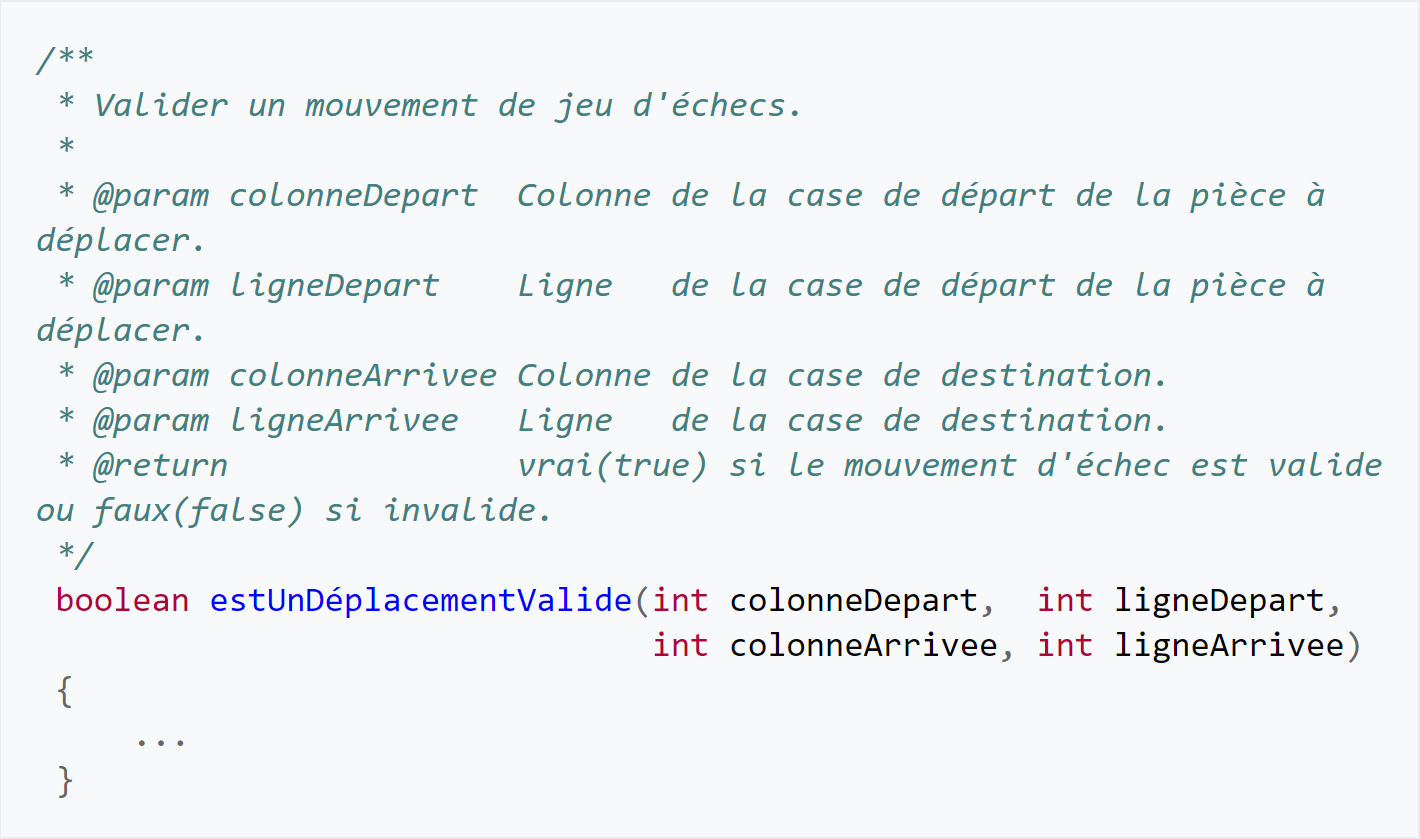
\includegraphics[scale=0.28]{Images/lol.png}
\end{frame}


\begin{frame}{Exemple avec Doxygen}
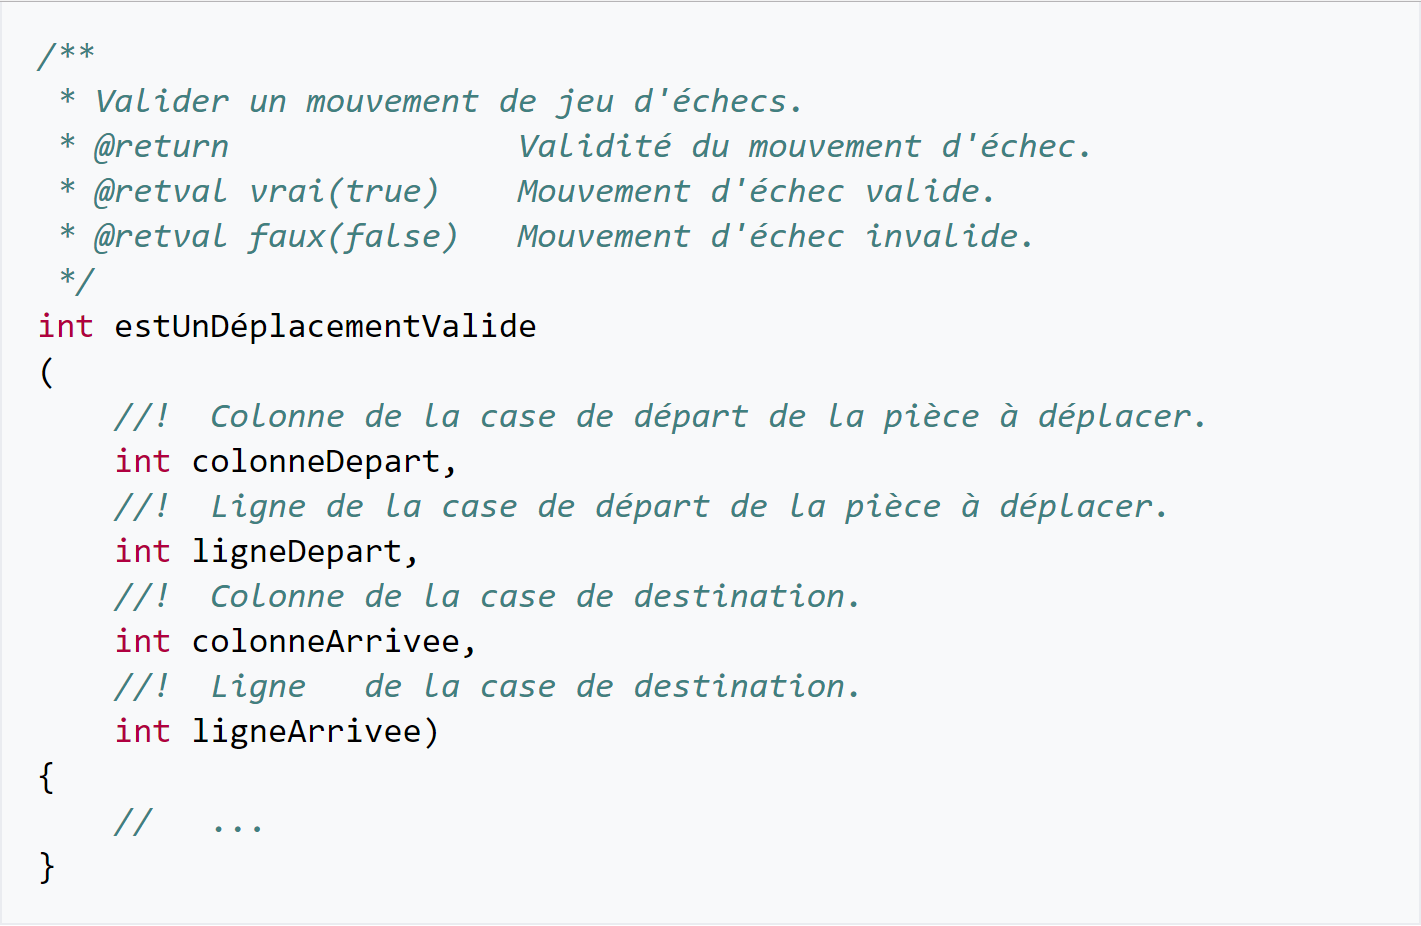
\includegraphics[scale=0.25]{Images/lol2.png}
\end{frame}










% SECTION SECTION SECTION SECTION !!!
% SECTION SECTION SECTION SECTION !!!
% SECTION SECTION SECTION SECTION !!!
\section{javadoc}

\subsection{Caractéristiques}
\begin{frame}{Caractéristiques}
\begin{itemize}
\item {
    Javadoc permet de creer une documentation d'api à partir des commentaires contenu dans son code java
}
\item {
    Pour que les blocs de commentaires soit reconnu par javadoc il doivent commencer par un "/**" et finir par un "*/", de plus chaque ligne commence par un "*".
}
\item {
    Il est possible de classifier les informations inclues dans les commentaires grâce a des tags specials 
}
\end{itemize}
\end{frame}




%EXEMPLE
\begin{frame}{Caractéristiques}
\begin{itemize}
\item {
    "@author" suivi de "bob" indiquera à javadoc que bob est
    l'auteur de cette partie du code et @version indique la version du code.
}
\end{itemize}
\begin{example}
    /** \\
    * @autor bob\\
    * @version 1.42\\
    */\\
    \\
    public class Kebab \\
    ...\\
    \\
\end{example}
\end{frame}

\subsection{Les tags}
\begin{frame}{Listes des tags et leurs fonctions}
 \begin{itemize}
  \item {
    @author Nom du développeur  
}
      \item {
@deprecated Marque la méthode comme dépréciée. Certains IDEs créent un avertissement à la compilation si la méthode est appelée.    
}
      \item {
@exception 	Documente une exception lancée par une méthode — voir aussi @throws.    
}
      \item {
@param 	Définit un paramètre de méthode. Requis pour chaque paramètre.    
}
      \item {
@return Documente la valeur de retour. Ce tag ne devrait pas être employé pour des constructeurs ou des méthodes définies avec un type de retour void.    
}

  \end{itemize}
\end{frame}




\begin{frame}{Listes des tags et leurs fonctions}
 \begin{itemize}
      \item {
@see Documente une association à une autre méthode ou classe.
}
          \item {
@since 	Précise à quelle version de la SDK/JDK une méthode a été ajoutée à la classe.  
}
          \item {
@throws	Documente une exception lancée par une méthode. Un synonyme pour @exception disponible depuis Javadoc 1.2.
}
          \item {
@version Precise la version du code
}
  \end{itemize}
\end{frame}


\begin{frame}{Generer la documentation}
 \begin{itemize}
    \item {
En general les EDI integrent une fonction qui permet à l'uttilisateur de generer la documentation facilement.
}
    \item {
Pour de la programmation en java on pourrai uttiliser l'EDI Eclipse
aller dans "projet" puis generer la doc;
}
  \end{itemize}
\end{frame}

\begin{frame}{Generer la documentation}
 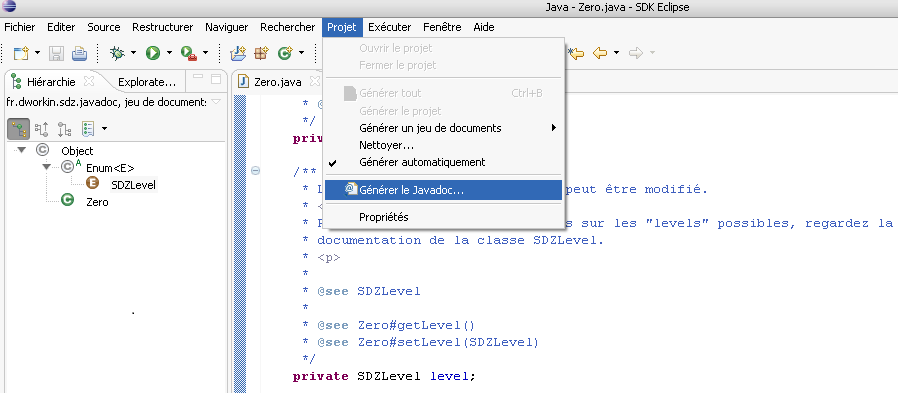
\includegraphics[scale=0.45]{Images/gendoc.png}
\end{frame}


\begin{frame}{Generer la documentation}
 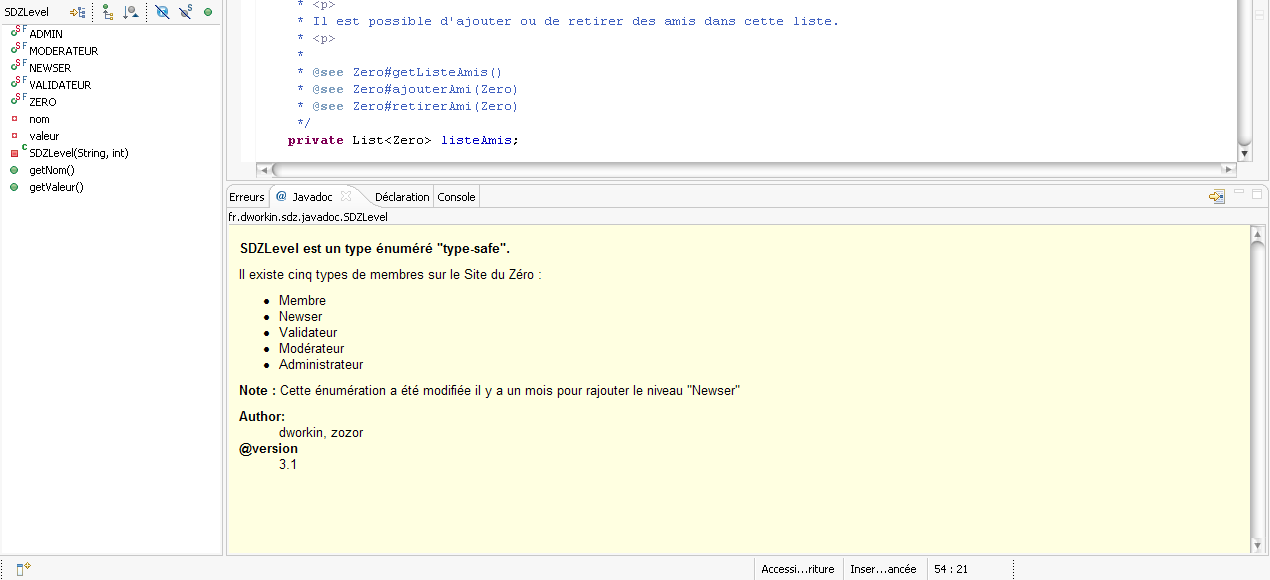
\includegraphics[scale=0.32]{Images/gendoc2.png}
\end{frame}

\begin{frame}{Generer la documentation}
\begin{itemize}
\item {
    On peut aussi uttiliser une ligne de commande avec javaDoc\\
}
\begin{example}
     javadoc  fichierSource.java -d doc
\end{example}
\item{
    Cette ligne va generer la documentation de fichierSource dans le dossier doc
}
\end{itemize}
\end{frame}

\subsection{Ccdoc et phpdoc ?}

\begin{frame}{Generer la documentation}
\begin{itemize}
    \item {
    Ccdoc et PHPdoc sont utillisées pour generer la documentation respectivement pour C/C++ et pour le PHP, leurs principe est exactemement le même que pour javadoc et reperent les commentaires de la meme maniere, (/**, *, @tag, */) ils sont d'ailleurs fortement inspirer de celui-ci.
}
\end{itemize}
\end{frame}


\begin{frame}{Ccdoc}
\begin{itemize}
    \item {
    On peut generer la documentation avec Ccdoc sur linux avec une ligne de commande:
    
    \begin{example}
    mkdir webdocs \\
    ccdoc -db documentation.db fichierSource.h -html webdocs/ \\
    \end{example}
}

\end{itemize}
\end{frame}


\begin{frame}{PHPdoc}
\begin{itemize}
    \item {
    Puis sur PHPdoc on peut faire de même:
    
    \begin{example} 
    phpdoc -d dossierDoc -f fichierSource.php
    \end{example}
}
\end{itemize}
\end{frame}


















% SECTION SECTION SECTION SECTION !!!
% SECTION SECTION SECTION SECTION !!!
% SECTION SECTION SECTION SECTION !!!
\section{Doxygen}

\subsection{Mais c'est quoi ?}
\begin{frame}{Mais c'est quoi ?}
 \begin{itemize}
  \item {
   A l'instar de Javadoc, Doxygen est un logiciel libre de documentation de code possédant des capacités de génération de documentation à partir du code source d'un programme. 
  }
  \item {
    Pour cela il tient compte de la syntaxe et de la structure du langage du programme ainsi que des commentaires associés à condition que ceux-ci soient écrit dans un format adapté. 
  }
  \end{itemize}
\end{frame}
\begin{frame}{Mais c'est quoi ?}
\begin{itemize}
    \item {
   La génération de documentation peut être faite à partir de code dans les langages suivants: C, C++, Java, Objective C, Python, IDL, VHDL et dans une certaine mesure PHP et D. 
    }
    \item{
    Le résultat final est une documentation complète générée en HTML (compressé ou non), LaTeX, RTF, PostScript, PDF avec hyperliens, et XML.
    }
    
\end{itemize}
\end{frame}

\begin{frame}{Mais c'est quoi ?}
\begin{itemize}
    \item {
   En permettant l'intégration de la documentation directement dans le code source, Doxygen permet de favoriser la cohérence entre la documentation et le code et de systématiser le comportement des développeurs afin qu'ils documentent le code qu'ils produisent.
    }
    \item{
  Il est également possible d'extraire de la documentation à partir d’un code source non documenté au préalable, ce qui peut faciliter la compréhension d'un programme dont le code est compliqué.
    }
    
\end{itemize}
\end{frame}


\subsection{Utilisation}
\begin{frame}{}
 \begin{itemize}
  \item {
   On va pouvoir voir différentes commandes et leur utilisations pour illustrer le fonctionnement de Doxygen.
   (Toutes les commandes doivent être précédées d'un  \backslash  )
  }
\end{itemize}
\end{frame}


\begin{frame}{a}
\begin{itemize}
  \item {
  Utiliser pour faire ressortir un paramètre dans sa description.
  }
\end{itemize}

\includegraphics[scale=0.20]Images/{m1.png} 

\end{frame}

\begin{frame}{bug}
\begin{itemize}
  \item {
  Utiliser pour indiquer un bug dans une fonction ou un morceau de programme.
  }
\end{itemize}


\includegraphics[scale=0.20]{Images/m2.png} 

\end{frame}

\begin{frame}{class [] []  }
\begin{itemize}
  \item {
  Utiliser pour décrire une classe. Le premier paramètre est obligatoire, les suivants optionnels. Attention toutefois à ce que les paramètres soit corrects, la casse est prise en compte.
  }
\end{itemize}

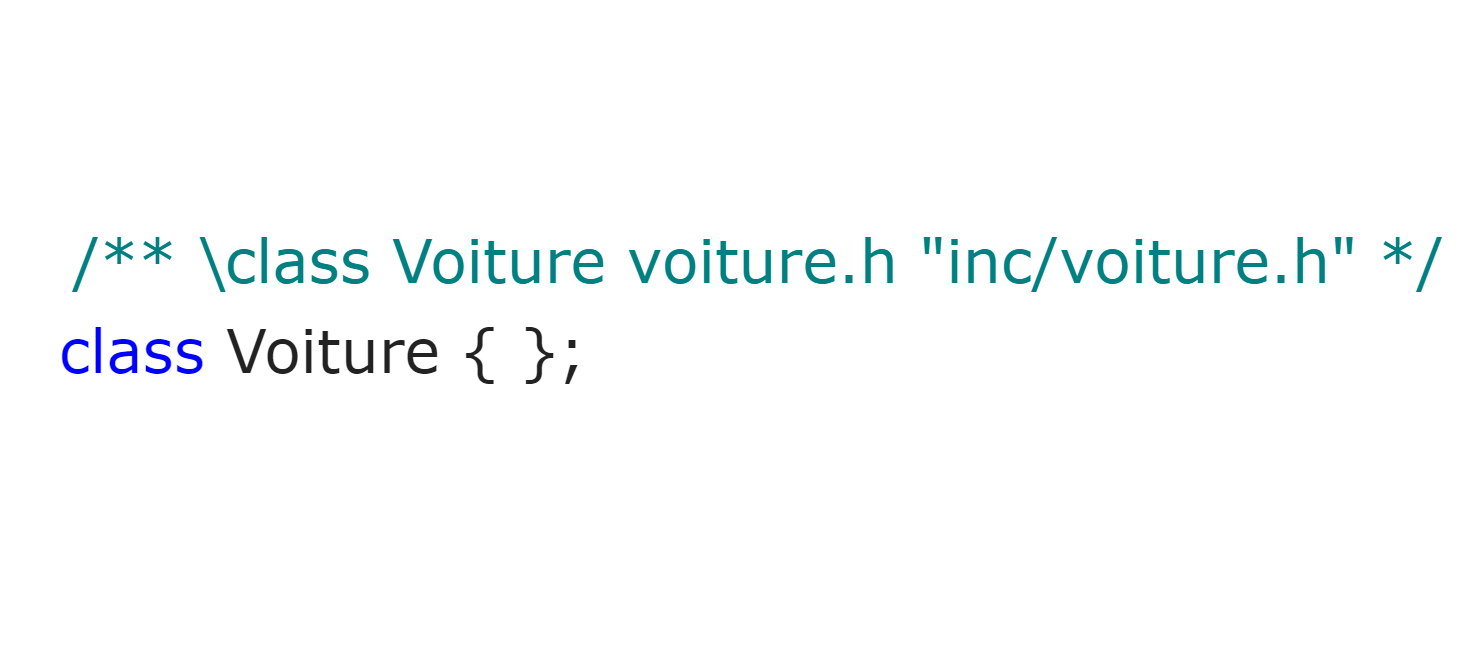
\includegraphics[scale=0.20]{Images/m3.png} 

\end{frame}

\begin{frame}{file }
\begin{itemize}
  \item {
  Utiliser pour décrire un fichier. L'attribut doit être exact et fourni avec l'extension.
  }
\end{itemize}

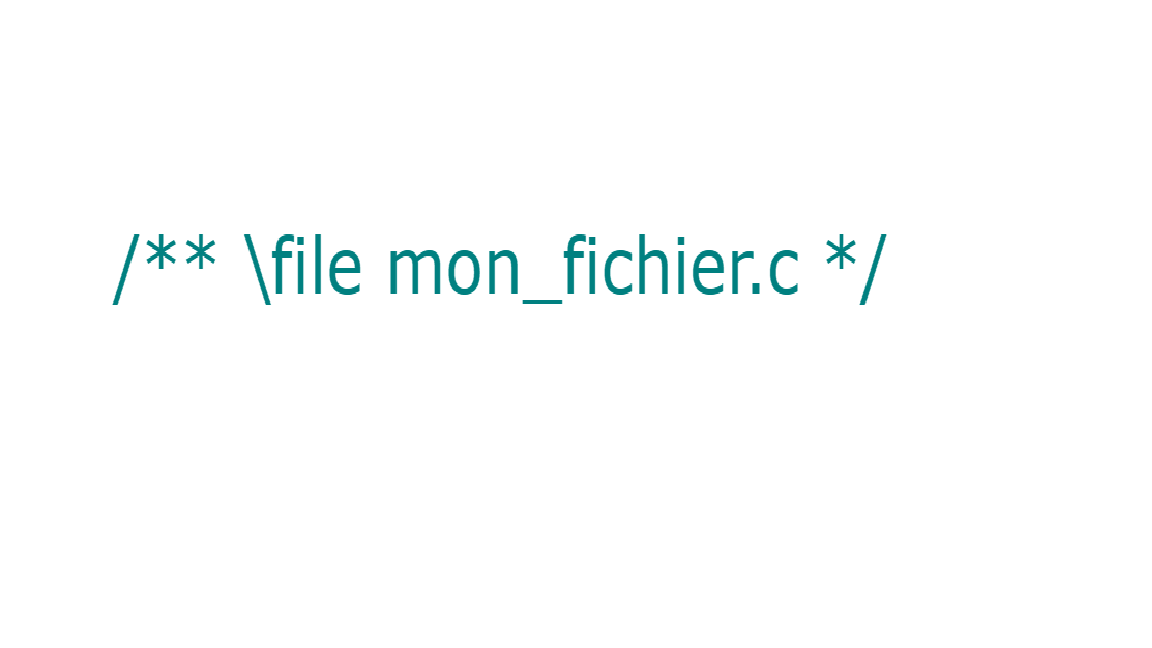
\includegraphics[scale=0.20]{Images/m4.png} 

\end{frame}

\begin{frame}{todo {description}}
\begin{itemize}
  \item {
  Utiliser pour indiquer ce qu'il reste à faire. La description peut être multiligne.
  }
\end{itemize}


\includegraphics[scale=0.20]{Images/m5.png} 

\end{frame}

\begin{frame}{typedef  }
\begin{itemize}
  \item {
  Utiliser pour introduire la description d'un typedef.
  }
\end{itemize}

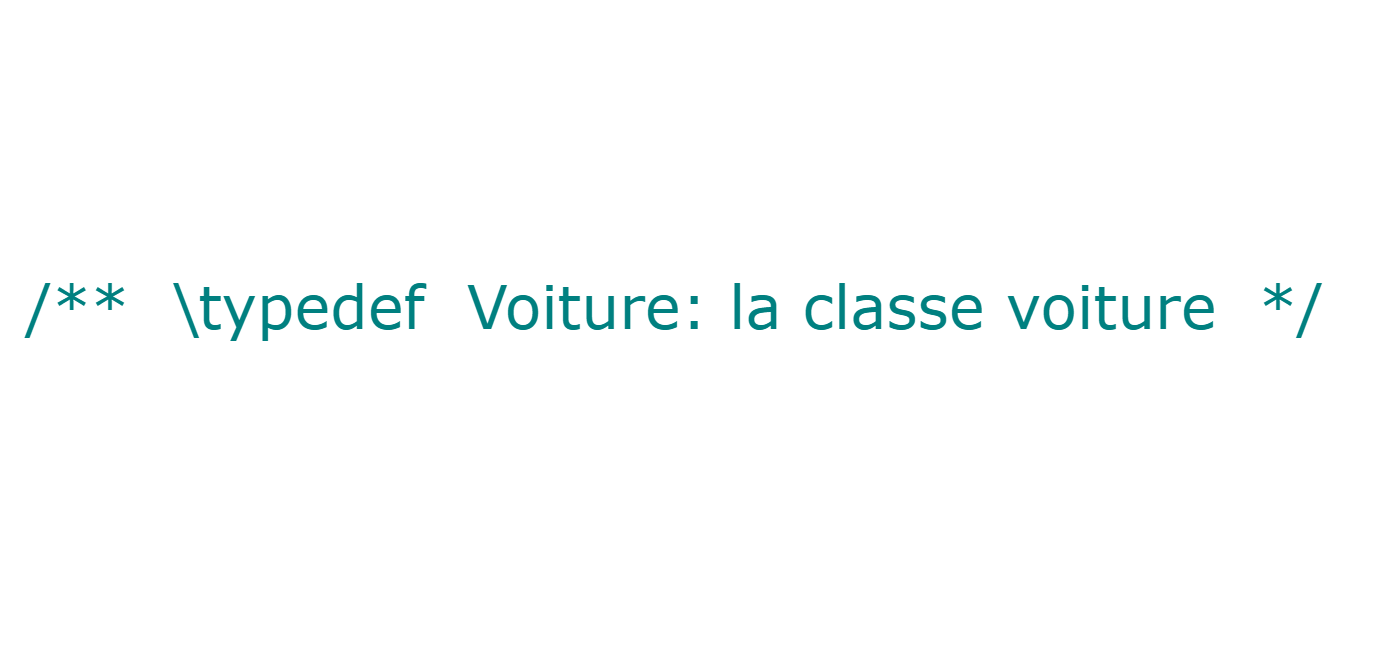
\includegraphics[scale=0.20]{Images/m6.png} 

\end{frame}

\begin{frame}{Exemple de résultat}
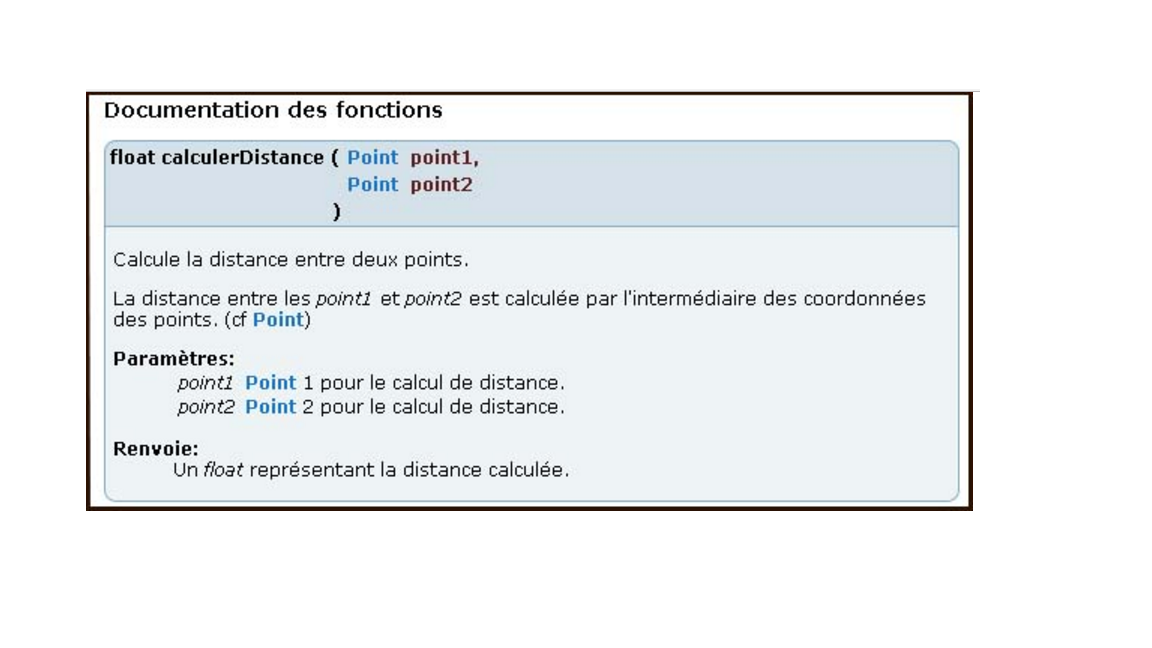
\includegraphics[scale=0.37]{Images/m12.png} 
\end{frame}

\begin{frame}{Fin}
\begin{itemize}
  \item {
  Merci d'avoir écouté !
  }
\end{itemize}
\end{frame}


% Placing a * after \section means it will not show in the
% outline or table of contents.
\section*{Summary}

\end{document}


